\section{La pregunta}

La Productividad Total de los Factores (PTF) no evolucionó de la misma manera
en todas las actividades económicas colombianas. Algunas registraron aportes
positivos durante buena parte de las dos últimas décadas. Otras tuvieron una
PTF negativa en la mayoría de los años. También hubo actividades que cambiaron
de signo entre subperiodos.

Este informe estudia la evolución de la PTF del total de la economía y de nueve
agregados de actividad económica entre 2005 y 2024. Compara tres dimensiones:
el aporte promedio durante todo el periodo, su persistencia anual y los cambios
entre cuatro subperiodos. El objetivo no es explicar cuánto creció cada
actividad, sino establecer cuándo la PTF contribuyó a ese crecimiento y cómo
cambió esa contribución.

La fuente es el anexo de Productividad Total de los Factores del DANE,
publicado bajo el enfoque de producción KLEMS. La serie reúne 19 variaciones
anuales, de 2006 a 2024, que enlazan los niveles de 2005 y 2024.

\section{Cómo se mide la PTF}

En el enfoque de producción, el crecimiento logarítmico de la producción de
cada actividad se descompone así:

\[
\Delta \ln Y =
\Delta \ln L + \Delta \ln K +
\Delta \ln E + \Delta \ln M + \Delta \ln S +
\Delta \ln PTF,
\]

donde $L$ corresponde a los servicios laborales; $K$, a los servicios de
capital; $E$, a energía; $M$, a materiales; y $S$, a servicios intermedios.
Cada aporte combina el crecimiento del insumo con su participación económica.

La PTF es la parte del crecimiento de la producción que no queda explicada por
los aportes medidos del trabajo, el capital y los insumos intermedios. Una PTF
positiva indica que la producción creció más que esos aportes. Una PTF negativa
indica que los aportes medidos crecieron más que la producción.

La PTF no es una medida pura de tecnología. El residuo puede incluir cambios
tecnológicos u organizacionales, pero también variaciones en la utilización de
capacidad, cambios de calidad no capturados y errores de medición. Por esta
razón, el informe describe la evolución de la PTF sin atribuir sus movimientos
a un mecanismo que los datos no identifican.

El total de la economía corresponde a la serie publicada por el DANE. No se
calcula como un promedio simple de las nueve actividades. De acuerdo con la
nota metodológica del anexo, el DANE pondera la agregación nacional con la
composición del valor agregado por actividad económica. Este informe usa
directamente el resultado agregado del DANE.

\subsection{El periodo correcto}

Los cuadros del DANE están rotulados por el año final de cada variación. La fila
2005 mide el cambio entre 2004 y 2005. Por tanto, la comparación entre los
niveles de 2005 y 2024 usa las variaciones de 2006 a 2024. El promedio de largo
plazo presentado en este informe corresponde a esas 19 observaciones.

\section{La PTF del total de la economía permaneció cerca de cero}

\begin{figure}[htbp]
\centering
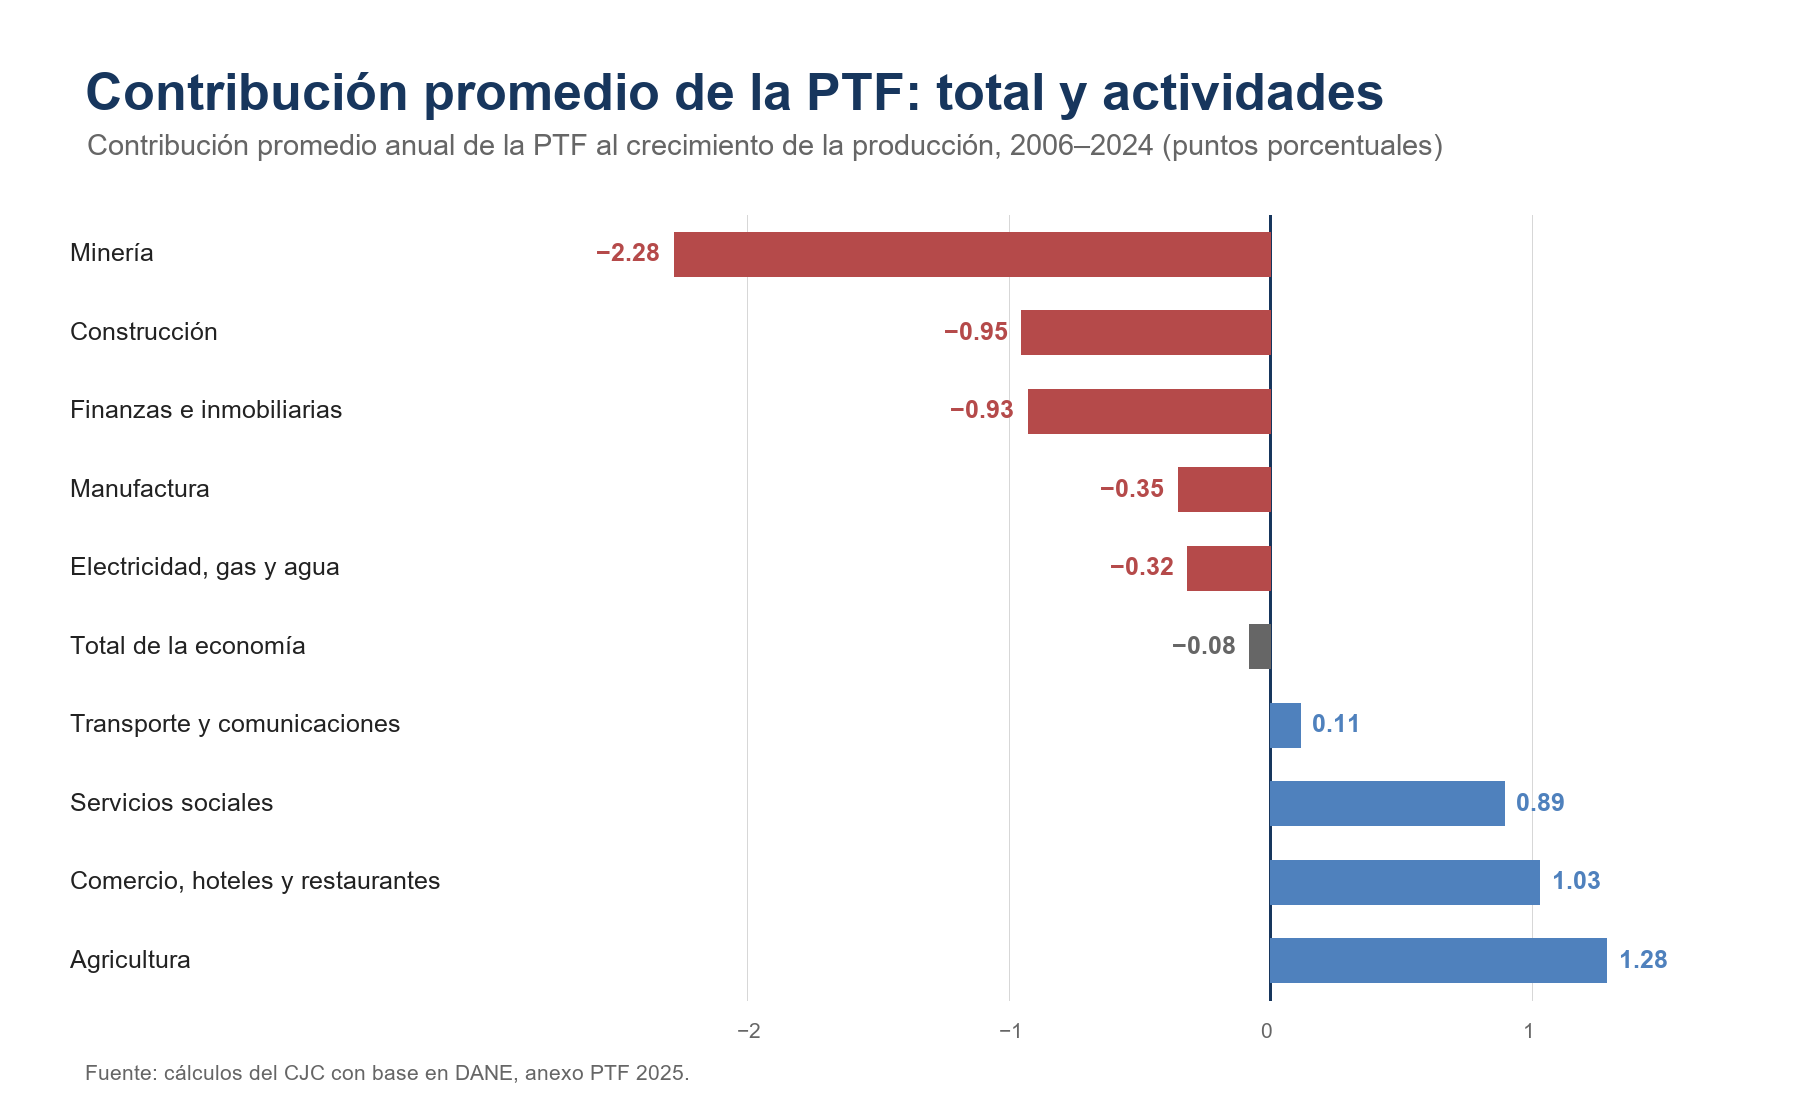
\includegraphics[width=\textwidth]{Paper/figures/fig_ptf_promedio_actividad.png}
\caption{Contribución promedio anual de la PTF del total de la economía y por actividad}
\label{fig:ptf_promedio}
\end{figure}

La PTF del total de la economía promedió $-0,08$ puntos porcentuales por año
entre 2006 y 2024. Ese resultado estuvo por debajo de agricultura, comercio,
servicios sociales y transporte, y por encima de las otras cinco actividades.
El valor cercano a cero no implica que las actividades tuvieran resultados
similares: los promedios sectoriales estuvieron entre 1,28 y $-2,28$ puntos.

La agricultura registró el mayor aporte promedio de la PTF:
1,28 puntos porcentuales por año. Le siguieron comercio, hoteles y restaurantes
con 1,03 puntos, y los servicios sociales, comunales y personales con 0,89.
Transporte, almacenamiento y comunicaciones tuvo un aporte positivo de
0,11 puntos, cercano a cero.

Las otras cinco actividades registraron una PTF promedio negativa. Minería
tuvo el menor aporte, con $-2,28$ puntos por año. Construcción registró
$-0,95$ puntos; finanzas e inmobiliarias, $-0,93$; manufactura, $-0,35$; y
electricidad, gas y agua, $-0,32$.

\newpage
El promedio de largo plazo permite ordenar las actividades, pero oculta cambios
importantes. El total de la economía pasó de un promedio negativo en
2006--2010 a valores cercanos a cero después de 2010. Agricultura tuvo un
promedio positivo a pesar de registrar una PTF negativa durante 2006--2010.
Electricidad, gas y agua tuvo un promedio negativo, aunque cambió a un aporte
positivo durante 2020--2024.

\section{La trayectoria cambió entre subperiodos}

\begin{figure}[htbp]
\centering
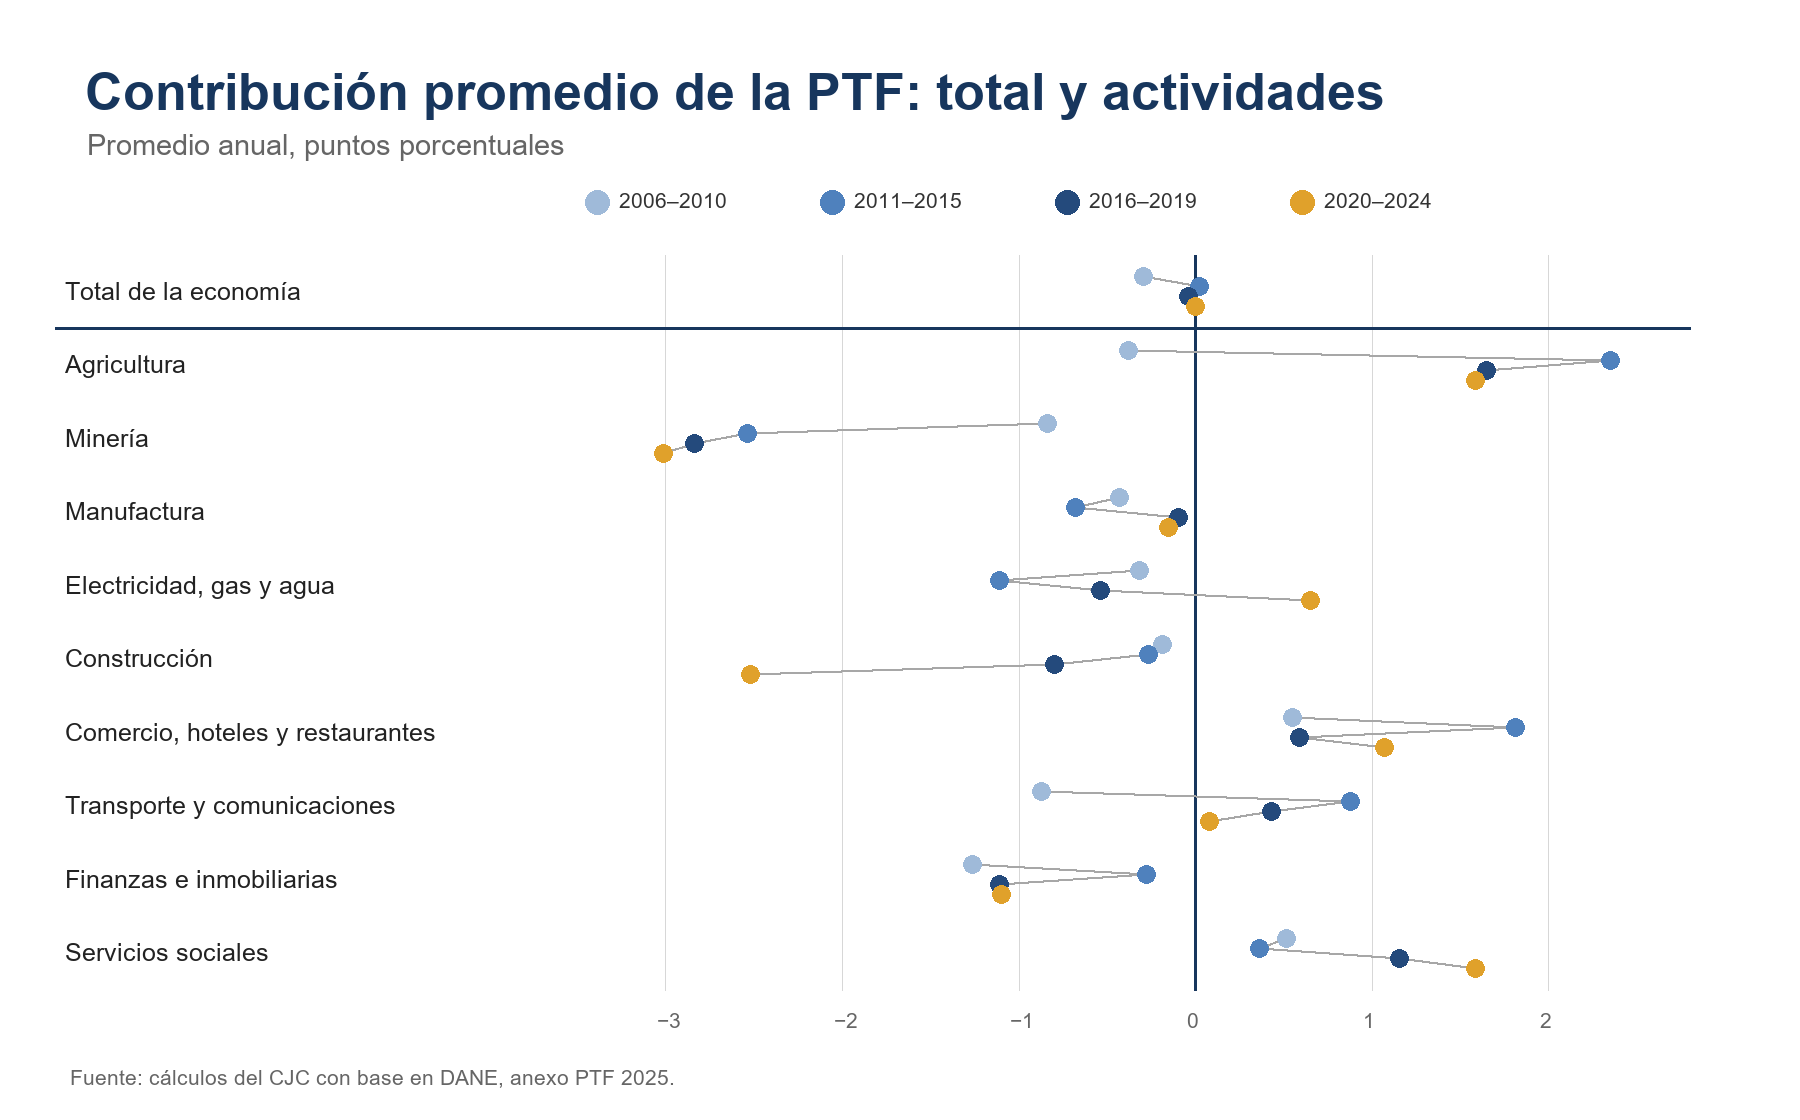
\includegraphics[width=\textwidth]{Paper/figures/fig_ptf_periodos_actividad.png}
\caption{Contribución promedio anual de la PTF del total de la economía y por actividad en cuatro subperiodos}
\label{fig:ptf_periodos}
\end{figure}

La Figura \ref{fig:ptf_periodos} compara cuatro promedios: 2006--2010,
2011--2015, 2016--2019 y 2020--2024. Los puntos unidos pertenecen a una misma
actividad. Un movimiento hacia la derecha indica un mayor aporte promedio de la
PTF; un cruce de la línea vertical indica un cambio de signo.

\begin{table}[htbp]
\centering
\caption{Evolución de la PTF por actividad y subperiodo}
\label{tab:evolucion_ptf}
\footnotesize
\begin{tabular}{p{3.8cm}rrrrr>{\centering\arraybackslash}p{1.3cm}}
\toprule
Actividad & 2006--10 & 2011--15 & 2016--19 & 2020--24 & 2006--24 & Años positivos \\
\midrule
Total de la economía & -0,30 & 0,02 & -0,04 & 0,00 & -0,08 & 10/19 \\
\midrule
Agricultura, ganadería, caza, silvicultura y pesca & -0,38 & 2,35 & 1,65 & 1,58 & 1,28 & 15/19 \\
Minería y extracción & -0,84 & -2,54 & -2,84 & -3,01 & -2,28 & 2/19 \\
Industrias manufactureras & -0,43 & -0,68 & -0,10 & -0,16 & -0,35 & 4/19 \\
Electricidad, gas y agua & -0,32 & -1,11 & -0,54 & 0,65 & -0,32 & 7/19 \\
Construcción & -0,19 & -0,27 & -0,80 & -2,52 & -0,95 & 7/19 \\
Comercio, hoteles y restaurantes & 0,55 & 1,81 & 0,59 & 1,07 & 1,03 & 14/19 \\
Transporte, almacenamiento y comunicaciones & -0,87 & 0,87 & 0,43 & 0,08 & 0,11 & 11/19 \\
Intermediación financiera, inmobiliarias, empresariales y de alquiler & -1,26 & -0,28 & -1,11 & -1,10 & -0,93 & 8/19 \\
Servicios sociales, comunales y personales & 0,51 & 0,36 & 1,16 & 1,59 & 0,89 & 14/19 \\
\bottomrule
\end{tabular}
\vspace{0.15cm}
\begin{minipage}{0.96\textwidth}
\footnotesize \textit{Nota:} contribución promedio anual de la PTF al crecimiento de la producción, en puntos porcentuales. El total de la economía corresponde a la serie agregada publicada por el DANE y no a un promedio simple de las actividades. Los subperiodos tienen distinta duración; se usan para describir cambios en la trayectoria, no para atribuirlos a un evento específico.
\par\textit{Fuente:} cálculos del CJC con base en DANE, anexo PTF 2025.
\end{minipage}
\end{table}


\subsection{El total pasó de un promedio negativo a valores cercanos a cero}

La PTF del total de la economía promedió $-0,30$ puntos por año en
2006--2010. El promedio fue de 0,02 puntos en 2011--2015, $-0,04$ en
2016--2019 y 0,00 en 2020--2024, después del redondeo. La PTF agregada pasó de
un promedio negativo a valores pequeños alrededor de cero. Uno de los tres
promedios posteriores a 2010 fue positivo y dos fueron levemente negativos.

La PTF del total fue positiva en 10 de 19 años y negativa en nueve. En 2024
aportó 0,62 puntos, después de restar 0,51 en 2023. La alternancia de signos
explica por qué los tres últimos promedios permanecieron cerca de cero.

\subsection{Agricultura pasó de una PTF negativa a aportes positivos}

La PTF de la agricultura fue de $-0,38$ puntos por año en 2006--2010. Pasó a
2,35 puntos en 2011--2015 y se mantuvo positiva en los dos subperiodos
siguientes: 1,65 puntos en 2016--2019 y 1,58 en 2020--2024. El cambio no
corresponde a un solo año. La agricultura registró una PTF positiva en todos
los años entre 2011 y 2021. Fue negativa en 2022 y volvió a ser positiva en
2023 y 2024.

En el conjunto del periodo, la agricultura tuvo una PTF positiva en 15 de
19 años. Esta combinación de magnitud y persistencia explica por qué ocupa el
primer lugar en el promedio de largo plazo.

\subsection{Comercio mantuvo un promedio positivo, con una caída en 2023}

Comercio, hoteles y restaurantes tuvo una PTF promedio positiva en los cuatro
subperiodos. El aporte pasó de 0,55 puntos en 2006--2010 a 1,81 en 2011--2015.
Después fue de 0,59 puntos en 2016--2019 y 1,07 en 2020--2024.

La trayectoria anual fue más volátil que esos promedios. La PTF alcanzó
6,42 puntos en 2021 y cayó a $-3,49$ en 2023. En 2024 fue de $-0,09$ puntos.
Por tanto, el promedio positivo de 2020--2024 combina una recuperación alta en
2021 con dos resultados negativos al final del subperiodo.

\subsection{Servicios sociales aumentó su aporte en los periodos recientes}

Los servicios sociales, comunales y personales también tuvieron una PTF
promedio positiva en los cuatro subperiodos. El aporte fue de 0,51 puntos en
2006--2010, 0,36 en 2011--2015, 1,16 en 2016--2019 y 1,59 en 2020--2024.

La PTF fue positiva en 14 de 19 años. En 2023 y 2024 aportó 3,47 y
2,74 puntos, respectivamente. A diferencia de comercio, los dos últimos años
mantuvieron el signo positivo del promedio reciente.

\subsection{Minería tuvo una PTF negativa en los cuatro subperiodos}

Minería fue la actividad con el resultado negativo más persistente. La PTF
promedio fue de $-0,84$ puntos en 2006--2010, $-2,54$ en 2011--2015,
$-2,84$ en 2016--2019 y $-3,01$ en 2020--2024. Solo dos de los 19 años
registraron una PTF positiva: 2009 y 2011.

El resultado de 2020, $-8,48$ puntos, redujo el promedio reciente. Sin embargo,
el signo negativo precede a la pandemia y se mantuvo entre 2021 y 2024. La
trayectoria de minería no puede explicarse únicamente por el choque de 2020.

\subsection{Manufactura permaneció cerca de cero, pero del lado negativo}

La PTF manufacturera fue negativa en los cuatro subperiodos: $-0,43$ puntos en
2006--2010, $-0,68$ en 2011--2015, $-0,10$ en 2016--2019 y $-0,16$ en
2020--2024. La cercanía a cero en los dos últimos promedios no significa
estabilidad anual. La PTF pasó de $-1,93$ puntos en 2020 a 3,97 en 2021 y
volvió a ser negativa entre 2022 y 2024.

Manufactura tuvo una PTF positiva en cuatro de 19 años. El promedio de largo
plazo fue menos negativo que el de minería, construcción o finanzas e
inmobiliarias, pero el signo positivo fue poco frecuente.

\subsection{Finanzas e inmobiliarias no consolidó un cambio de signo}

La PTF del agregado financiero e inmobiliario fue negativa en los cuatro
subperiodos. El promedio pasó de $-1,26$ puntos en 2006--2010 a $-0,28$ en
2011--2015, pero volvió a $-1,11$ en 2016--2019 y fue de $-1,10$ en
2020--2024.

La PTF fue positiva en tres de los últimos cinco años. Sin embargo, la caída de
$-6,70$ puntos en 2021 mantuvo negativo el promedio reciente. Como el agregado
incluye intermediación financiera, actividades inmobiliarias, empresariales y
de alquiler, el resultado no debe atribuirse exclusivamente al sistema
financiero.

\subsection{Electricidad cambió de signo; construcción se deterioró}

Electricidad, gas y agua pasó de promedios negativos en los tres primeros
subperiodos a 0,65 puntos en 2020--2024. La PTF fue positiva entre 2021 y 2024,
después de registrar $-0,88$ puntos en 2020. Es el cambio de signo más claro
del periodo reciente.

Construcción siguió la dirección contraria. La PTF promedio fue de
$-0,19$ puntos en 2006--2010, $-0,27$ en 2011--2015 y $-0,80$ en
2016--2019. En 2020--2024 cayó a $-2,52$ puntos. El resultado está afectado
por la caída de $-9,76$ puntos en 2020, pero la PTF también fue negativa en
2021 y 2023.

\subsection{Transporte mejoró después de 2010, sin sostener un aporte alto}

Transporte y comunicaciones pasó de $-0,87$ puntos en 2006--2010 a
0,88 puntos en 2011--2015. El promedio disminuyó a 0,43 puntos en
2016--2019 y a 0,08 en 2020--2024. La actividad mejoró frente al primer
subperiodo, pero no consolidó un aporte positivo de magnitud creciente.

La PTF cayó a $-2,50$ puntos en 2023 y subió a 1,15 en 2024. Esa reversión
explica por qué el promedio reciente terminó cerca de cero.

\section{La serie anual muestra persistencia y choques}

\begin{figure}[htbp]
\centering
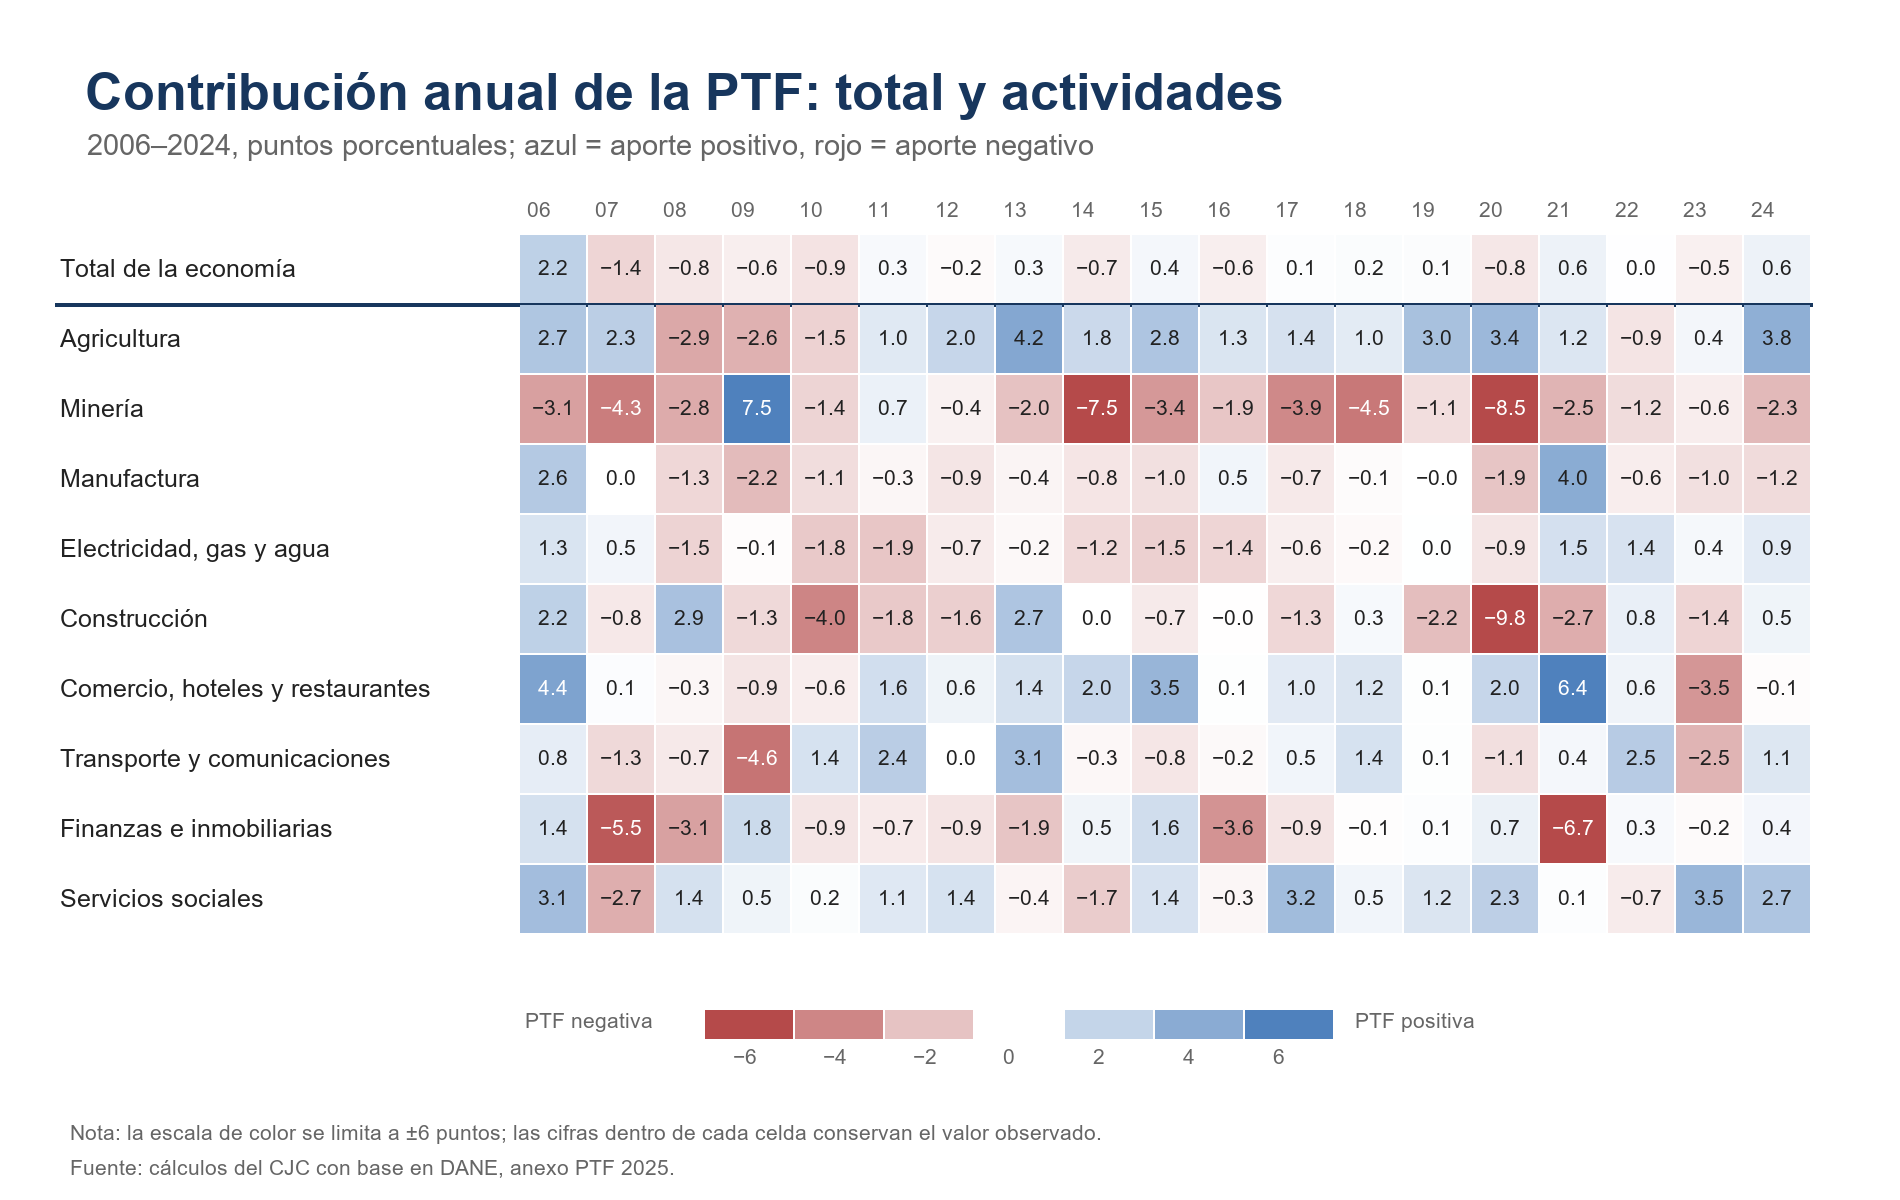
\includegraphics[width=\textwidth]{Paper/figures/fig_ptf_mapa_anual.png}
\caption{Contribución anual de la PTF del total de la economía y por actividad}
\label{fig:ptf_mapa}
\end{figure}

La Figura \ref{fig:ptf_mapa} presenta el valor anual de la PTF. Las celdas
azules indican aportes positivos y las rojas, aportes negativos. La intensidad
del color aumenta con la magnitud. La figura permite distinguir un resultado
persistente de un promedio dominado por uno o dos años extremos.

La primera fila muestra que la PTF del total de la economía alternó entre
valores positivos y negativos. El aporte anual estuvo entre 2,21 puntos en
2006 y $-1,39$ en 2007. Desde 2011, todos los valores se ubicaron entre
$-0,78$ y 0,62 puntos.

Agricultura, comercio y servicios sociales acumularon 15, 14 y 14 años
positivos, respectivamente. Minería tuvo 17 años negativos y manufactura, 15.
Electricidad, construcción y finanzas e inmobiliarias tuvieron 12, 12 y
11 años negativos. Transporte fue la actividad más dividida: 11 años positivos
y ocho negativos.

\subsection{La pandemia amplificó la volatilidad}

En 2020, construcción y minería registraron las caídas más grandes de toda su
serie: $-9,76$ y $-8,48$ puntos. En 2021, comercio alcanzó 6,42 puntos y
manufactura 3,97, mientras finanzas e inmobiliarias cayó a $-6,70$. Estos
movimientos afectan los promedios de 2020--2024 y dificultan interpretar ese
subperiodo como una tendencia estable.

La PTF del total de la economía fue de $-0,78$ puntos en 2020 y 0,61 en 2021.
Después aportó 0,04 puntos en 2022, restó 0,51 en 2023 y aportó 0,62 en 2024.
El promedio 2020--2024 fue 0,00 porque los años positivos y negativos se
compensaron.

El choque pandémico no explica todos los signos de largo plazo. Minería,
manufactura y finanzas e inmobiliarias ya tenían promedios negativos antes de
2020. Agricultura, comercio y servicios sociales ya registraban promedios
positivos.

\subsection{En 2024 aumentó la PTF del total y de seis actividades}

Entre 2023 y 2024, la PTF del total de la economía pasó de $-0,51$ a
0,62 puntos. También aumentó en seis de las nueve actividades. Los
mayores aportes en 2024 fueron los de agricultura (3,80 puntos), servicios
sociales (2,74), transporte y comunicaciones (1,15) y electricidad, gas y agua
(0,94). Construcción y finanzas e inmobiliarias también tuvieron aportes
positivos, de 0,53 y 0,41 puntos.

Manufactura y minería mantuvieron una PTF negativa en 2024, con $-1,20$ y
$-2,33$ puntos. Comercio pasó de $-3,49$ puntos en 2023 a $-0,09$ en 2024:
mejoró, pero no cambió de signo. Un solo año no modifica la clasificación de
largo plazo, aunque sí muestra que las posiciones sectoriales pueden cambiar
con rapidez.

\section{Qué añade la descomposición de los factores}

El foco de este informe es la evolución de la PTF. La descomposición de trabajo,
capital, energía, materiales y servicios se presenta en los apéndices para
aclarar qué significa un residuo positivo o negativo.

En minería, por ejemplo, el capital aportó 2,99 puntos por año entre 2006 y
2024, mientras la PTF restó 2,28. En finanzas e inmobiliarias, el capital
aportó 2,04 puntos y la PTF restó 0,93. Estos resultados muestran que un aporte
alto del capital no coincidió con una PTF positiva.

En agricultura, la PTF aportó 1,28 puntos y explicó 49\% del crecimiento
promedio de la producción. En comercio explicó 28\% y en servicios sociales,
19\%. La descomposición ayuda a dimensionar la PTF, pero no identifica qué
cambios tecnológicos, organizacionales o de medición explicaron su trayectoria.

\section{Implicaciones}

\textbf{El promedio del total no describe la dispersión sectorial.} La PTF del
total de la economía promedió $-0,08$ puntos, mientras los promedios por
actividad estuvieron entre 1,28 puntos en agricultura y $-2,28$ en minería.
El total publicado incorpora las ponderaciones del DANE y no debe interpretarse
como el desempeño de una actividad representativa.

\textbf{El promedio de largo plazo debe acompañarse con una medida de
persistencia.} Agricultura y comercio tuvieron aportes promedio similares,
pero sus últimos años fueron distintos. Agricultura cerró 2024 con 3,80 puntos;
comercio, con $-0,09$. El número de años positivos y la trayectoria reciente
evitan interpretar el promedio como un resultado constante.

\textbf{Los cambios de signo requieren seguimiento.} Electricidad, gas y agua
tuvo una PTF positiva entre 2021 y 2024 después de tres subperiodos con
promedios negativos. Construcción registró el movimiento contrario en
2020--2024. La publicación de nuevos años permitirá establecer si esos cambios
persisten o responden a la volatilidad posterior a la pandemia.

\textbf{La PTF no identifica por sí sola la causa de una trayectoria.} El
resultado permite localizar actividades y periodos que requieren una
explicación adicional. Determinar la causa exige información sectorial sobre
producción e insumos que no está contenida en el residuo.

\textbf{El DANE debería publicar la serie en formato longitudinal.} Los cuadros
anuales permiten reconstruir la evolución, pero exigen enlazar veinte hojas.
Una base única, con metadatos sobre revisiones y correspondencias entre
clasificaciones, permitiría distinguir una revisión estadística de un cambio
económico.

\section{Conclusión}

La PTF del total de la economía promedió $-0,08$ puntos por año entre 2006 y
2024. Después del promedio de $-0,30$ puntos en 2006--2010, los tres
subperiodos siguientes permanecieron cerca de cero. Este resultado agregado
coexistió con promedios sectoriales entre 1,28 y $-2,28$ puntos.

Agricultura, comercio y servicios sociales registraron aportes positivos y
frecuentes entre 2005 y 2024. Minería, manufactura y finanzas e inmobiliarias
tuvieron promedios negativos en los cuatro subperiodos. Electricidad cambió de
signo, construcción cayó a $-2,52$ puntos en 2020--2024 y transporte terminó
cerca de cero.

La PTF de la agricultura pasó de $-0,38$ puntos en
2006--2010 a promedios superiores a 1,5 puntos en los tres subperiodos
siguientes. Minería registró el deterioro más persistente y construcción, la
mayor caída reciente. Electricidad fue la única actividad que pasó de tres
subperiodos negativos a un promedio positivo en 2020--2024.

El resultado de 2024 fue mejor que el de 2023 para el total de la economía y
para seis actividades. Los próximos años mostrarán si el total consolida un
aporte positivo, si agricultura y servicios sociales sostienen sus resultados,
si electricidad conserva el cambio de signo y si construcción, manufactura y
minería interrumpen sus trayectorias negativas.
